\section{eBPF Setup}\label{sec:ebpf_setup}

This section will discuss which eBPF programs are needed to realize the wanted 
relay functionality within the Linux kernel, as well as their individual 
responsibilities.

\subsection{Different eBPF Programs}

In order to allow the relay to forward packets independently of the userspace, we
need to equip the relay with three eBPF programs, as seen in~\autoref{fig:ebpf-programs}.
Those three programs are:

\begin{itemize}
    \item a program that handles incoming traffic \textbf{from} the clients (client ingress)
    \item a program that handles incoming traffic \textbf{from} the video server (server ingress)
    \item a program that handles outgoing traffic \textbf{to} the clients (client egress)
\end{itemize}
Their responsibilities then are:

\begin{itemize}
    \item handling the initial registration of new clients and storing their information, such as
    MAC addresses in an eBPF map
    \item intercepting the packets from the video server, duplicating and redirecting them to 
    the egress program (as well as sending one unaltered packet to userspace for state
    management purposes)
    \item receiving the redirected packets at egress, altering them using the client-specific
    data, deciding (based on packet priority and client congestion) if a packet should be dropped 
    or sent, storing info on sent-out packets for future congestion control purposes, and finally, sending 
    them out to the clients
\end{itemize}
This setup allows us to separate any state management and congestion control from the actual
packet forwarding and thus makes leaving out any immediate userspace processing possible.

\vspace{0.5cm}
\begin{figure}[H]
    \centering
    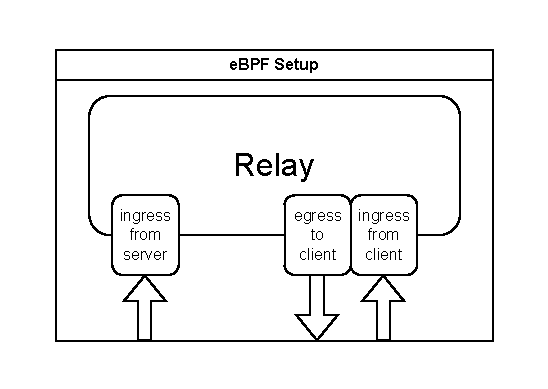
\includegraphics[width=0.4\textwidth]{figures/03_fast_relays/ebpf-setup.drawio.pdf}
    \caption[Types of eBPF programs at relay]{The relay has to be equipped with three eBPF programs.}\label{fig:ebpf-programs}
\end{figure}

Following is a more detailed description of the responsibilities of each of the three programs.
\subsubsection{Client Ingress} 
This ingress eBPF program initially does some simple packet inspection on every incoming packet 
looking if the packet uses the correct protocols and addresses the right application layer.
This is done by initially parsing the Ethernet, IP, and UDP headers, if present, and checking if 
the port matches the one the relay application is listening on.
This means the correct port is to be defined prior such that the eBPF program can associate 
a single or (multiple) relay instance(s) with the correct port.
In our case, then, since we use QUIC, the program will check for QUIC long header packets that 
setup an initial connection and save the transmitted state information such as connection-id, 
stream-related states, et cetera, in an eBPF map together with information that is not directly known
by the userspace, such as the client's MAC address.
Saving data like the MAC address directly once the connection is set up allows us to omit any further 
Address Resolution Protocol (ARP) steps later on. 
\subsubsection{Server Ingress}
Another ingress-related program, this time for packets coming from the video server, is needed
to handle packet duplication and forwarding.
This program will receive the actual video packets from the server and then, based on an internal 
counter of how many clients actually want to receive the video, duplicate the packets accordingly.
The counter indicating the number of clients will be updated by the userspace once a new connection 
is fully established and the client is ready to receive the actual video data.
This might potentially cause some minuscule delay when updating the counter, but sending cached 
video data to the client for a brief moment when updating the counter could be a solution. % TODO: needed?
\autoref{fig:packet-forwarding-duplication} shows the high-level packet duplication and forwarding process 
for an example with three clients that want to receive the video data.

In this ingress program, we need to consider a few things to ensure the correctness
of our approach.
These are:
\begin{enumerate}
    \item   The program can \textbf{only} forward packets that contain video data and must not 
            forward any other packets that contain e.g.~control data.

    % \begin{enumerate}
            This is fairly easy to achieve by doing some header inspection of the QUIC header,
                which contains the packet type. Also, since the payload is generally sent using 
                short-headers, there is no need to consider long-header packets.
    % \end{enumerate}

    \item   The program should pass an unaltered copy of each packet up to userspace to allow the 
            QUIC library to gain knowledge of the packet and handle any state changes accordingly.

    % \begin{enumerate}
            Generally speaking, this is not strictly necessary, as one could just have a separate 
                setup of registering packets that came from the server, but as this is not needed,
                it is considerably easier to just pass the packet up to userspace and let the 
                library handle it normally. This does not impose any additional overhead as the
                forwarding of any duplicate packets happens independently, of course.

            Any packet that has been identified as not part of our dataflow should, of course, 
                be passed up to userspace without being forwarded to egress.
    % \end{enumerate}
\end{enumerate}

\begin{figure}[htbp]
    \centering
    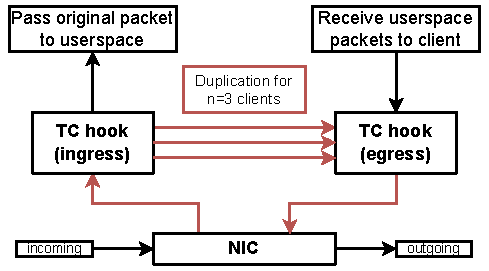
\includegraphics[width=0.5\textwidth]{figures/03_fast_relays/packet-forwarding.drawio.pdf}
    \caption[Video packet duplication]{Duplication and forwarding of video packets to egress directly 
    from ingress.}\label{fig:packet-forwarding-duplication}
\end{figure}

Duplicating and forwarding incoming packets that were identified as containing payload can be done 
using \verb|bpf_clone_redirect(skb, egress_ifindex, 0)| which is a helper function
that allows one to clone the packet buffer provided as the first argument and add it to the 
queue of the interface with the index that is provided as the second argument.
The last argument allows for the specification of additional flags.
Aside from \verb|bpf_clone_redirect|, there are also other helper functions regarding packet
redirection with slightly different behavior, so it is crucial to choose the appropriate one
to get the desired outcome~\parencite{bpf-helpers-man-page,eBPF-redirects-types}.
\autoref{tab:skb-redirection} shows them together with a brief description of their behavior.

\begin{table}[H]
    \centering
    \begin{tabular}{L{7cm}L{7cm}}
        \toprule
            Helper & Description \\
        \midrule
            \verb|bpf_clone_redirect| & Clones and redirects a packet to the interface associated with the provided index.\\
        \midrule
            \verb|bpf_redirect| & Redirects a packet to the interface associated with the provided index. The packet is not cloned 
                                    (no underlying call of \verb|skb_clone()|) so it is slightly more efficient.
                                    % (25\% pps increase according to commit message). % TODO: find commit message
                                    The packet is also not redirected immediately but after the function finishes.\\ 
        \midrule
            \verb|bpf_redirect_peer| & Similar to \verb|bpf_redirect|, but instead of redirecting the packet to the interface provided 
                                        as a parameter, it is redirected to its peer device. This works only between different netns to 
                                        allow for an efficient ``ingress to ingress netns switch''. The switch is more performant since 
                                        the packet does not need to go through the CPU backlog queue.\\ % TODO: what does the CPU backlog queue do?
        \midrule
            \verb|bpf_redirect_neigh| & Again similar to \verb|bpf_redirect| but allows to redirect a packet to another net device. 
                                        This helper also fills in all the correct L2 addresses of the neighboring subsystem. 
                                        Internally this executes a neighbor lookup to find the needed L2 information. \\
        \bottomrule
    \end{tabular}
    \caption[Redirection helpers for packet buffer]{Helper functions for packet redirection.
    There are more than that, but those are the ones we identified as possibly useful 
    initially.}\label{tab:skb-redirection}
\end{table}

Based on the descriptions of the redirection helper functions mentioned in~\autoref{tab:skb-redirection}
it becomes clear that \verb|bpf_clone_redirect| is the one suitable for our use case. 
This is because we need the cloning aspect since we essentially want to duplicate the incoming packets multiple times.
Also, the redirection to another namespace or another net device, as provided by \verb|bpf_redirect_peer| and
\verb|bpf_redirect_neigh|, respectively, is not needed in our case since we operate in the same relay-namespace
throughout the whole process.

\subsubsection{Client Egress}\label{sec:client-egress}
The central part of the eBPF setup where everything, from state-management to packet forwarding, 
comes together is the program that handles the outgoing traffic towards the clients.
The client egress program sees every packet that leaves the relay, which includes packets that have 
been redirected by the ingress program as well as packets that have been generated by the relay itself
(i.e.~come from the relay userspace).
This means that the program essentially merges two streams of packets into one stream that needs to 
be in a consistent state.
This interleaving of packets grows the requirements of the program to the following list.
% Bold numbers indicate that a requirement is caused by the interleaving of packets.
The second and third requirements are directly caused by the interleaving of packets, while the other points are
general requirements for the egress program.
\begin{enumerate}
    \item[1.]   Obviously, similar to the other eBPF programs, any packet that is not part of our traffic 
            should be passed on normally without any further processing.
    \item[2.] In case the packet is QUIC (for the correct client connection), the packet-number 
            needs to be changed to a program internal counter to avoid issues of reusing packet-numbers. 
            This is the only place where we can guarantee sequential packet-numbers since neither 
            the userspace nor the server knows what the highest packet-number sent at any moment in time is. 
            As there is no way of synchronizing lookups (e.g.~using eBPF maps) of information between userspace 
            and an eBPF program, changing it right before sending it out is the best way of keeping them coherent. 
    \item[3.] In case the packet (in addition to being QUIC for a client connection) contains 
                        stream frames, we need to do a similar translation of the stream-id.
                        The reasons and methods for this are the same as for the packet-number translation.
                        \autoref{fig:stream-id-translation} shows a flow diagram of the stream-id translation
                        process.
                        Important steps include checking if the stream-id translation already exists as well
                        as figuring out where a stream was created.
                        The former is necessary in case a payload is split into multiple packets, and the latter is 
                        necessary since the relay essentially has a fan in of two (relay originated packets and 
                        server-originated packets).
                        This fan-in might cause a situation where both the relay and the server open a stream which 
                        initially has the same id (since the server and relay states are not synchronized).
                        In such a case, the two streams must not be mapped to the same outgoing stream-id.  
                        This is also why a retransmission coming from the relay needs to be treated as 
                        if it came from the server. For that the eBPF program will be notified by the userspace 
                        regarding which packets are such retransmissions.
    \item[4.] Again, if the packet is QUIC and for the right connection, the program needs 
                        to read the packet's priority and decide via a map-lookup if the connection 
                        state allows sending packets with the given priority.
    \item[5.] If the packet is a redirected media stream data packet, the program must determine 
            which client it should be sent to. 
            This is done by saving the client id in some part of the packet that will be 
            overwritten at egress (namely the connection-id) before redirecting the packet.
            The egress program, knowing where the id is saved in case of a redirected packet, can then
            lookup the correct address data of the client (i.e.~MAC address, IP address, etc.) using 
            the saved id and overwrite the respective fields in the buffer before sending it out.
\end{enumerate}
\vspace{0.5cm}
\begin{figure}[H]
    \centering
    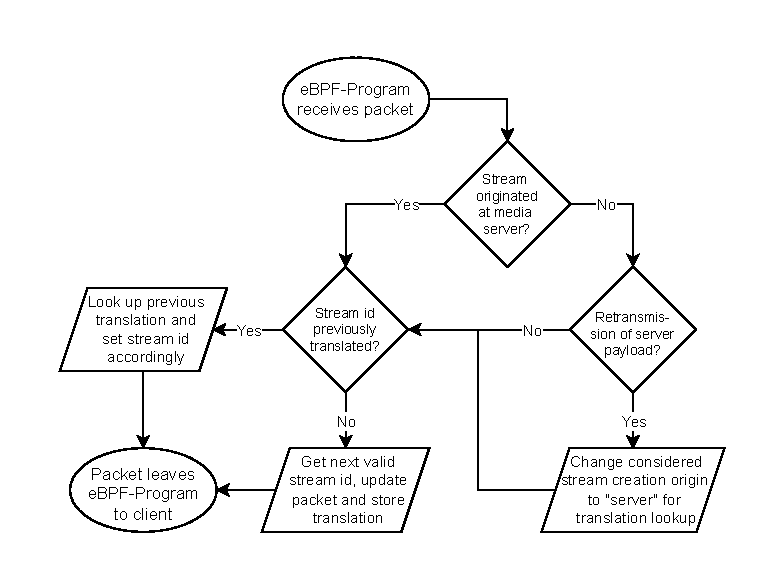
\includegraphics[width=0.7\textwidth]{figures/03_fast_relays/stream-id-translation.drawio.pdf}
    \caption[Stream-id translation schematic]{Flow diagram of stream-id translation process.}\label{fig:stream-id-translation}
\end{figure}
% Since the QUIC protocol works with packet-numbers for a given connection, it is necessary for 
% the egress program to make sure the forwarded packets together with the userspace packets
% provide a consistent state. 
% For this, the egress program maintains its own packet-number counter for each connection.
% That way, only one counter has to be maintained, and race conditions can be avoided.
The aforementioned packet-number translation means that the packets sent by the userspace will likely have a different packet-number i.e.~not the one chosen by the QUIC library.
This might lead to inconsistencies again when receiving ACKs but can be avoided by 
remembering the translation in a map as well as only storing packet objects in the 
Go library that have the correct state.
This technique of ``storing'' a packet that the userspace does not know
about, since it comes from the media server, will be referred to as ``packet registration''.
This initially gives a brief window where a packet was sent out but is not saved in the history
of the QUIC library.
Once the packet is then processed by the userspace routine handling the 
registration, any incoming ACKs for this packet can be processed correctly.
The next section will go into more detail on how the packet registration works.
Later, we will also look at the implications of this on retransmissions.
Even though the stream-id translation works very similarly to the packet-number translation, it 
does not have the need for any additional work after the packet has been sent out since our 
approach uses unidirectional streams only, and thus the relay does not care about changes in 
the used stream-id. % TODO: maybe reorder the sentences a little bit

\subsection{Packet Registration}
In order to make the congestion control algorithm, which is running in userspace,
usable, we need to inform the QUIC library about the forwarded packets.
This again happens via eBPF maps and a separate go routine that continuously
polls new entries in the map and processes them.
Entries are then added to the packet history to allow the receipt of ACKs.
Besides that, the congestion control algorithm will be informed about the
forwarded packet in order to be able to react to potential congestion events.
\autoref{fig:forward-registration} visualizes the setup for this process.
\vspace{0.5cm}
\begin{figure}[H]
    \centering
    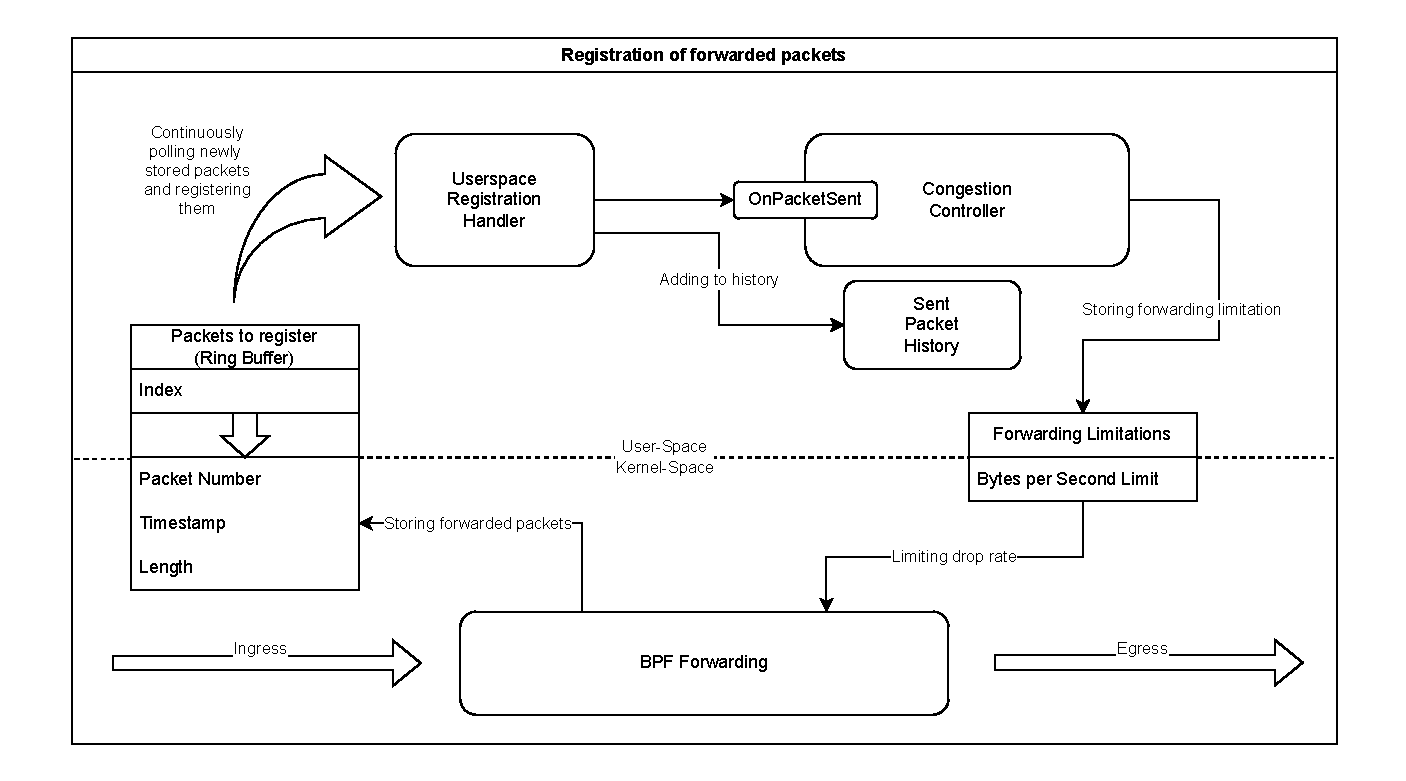
\includegraphics[width=0.7\textwidth]{figures/03_fast_relays/forward-registration.drawio.pdf}
    \caption[Packet registration schematic]{Internal setup for registering forwarded packets as well as incorporating forwarding
    limitations for the BPF program.}\label{fig:forward-registration}
\end{figure}

\subsection{Retransmissions of Forwarded Packets}
The fact that the relay only knows about the packets after a separate registration call causes 
another issue when it comes to retransmissions.
Retransmissions happen at a stream level, which means that the relay needs to know about the 
stream in the first place if it wants to retransmit a packet.
Given that we actually never create the streams that contain the frames of the payload data 
at the relay, this is a problem.
Our proposed system handles this by manually creating a stream with the correct id, the first
time a packet goes missing for that stream.
This can be imagined as a ``just-in-time'' stream creation before the retransmission is sent.

\begin{figure}[H]
    \centering
    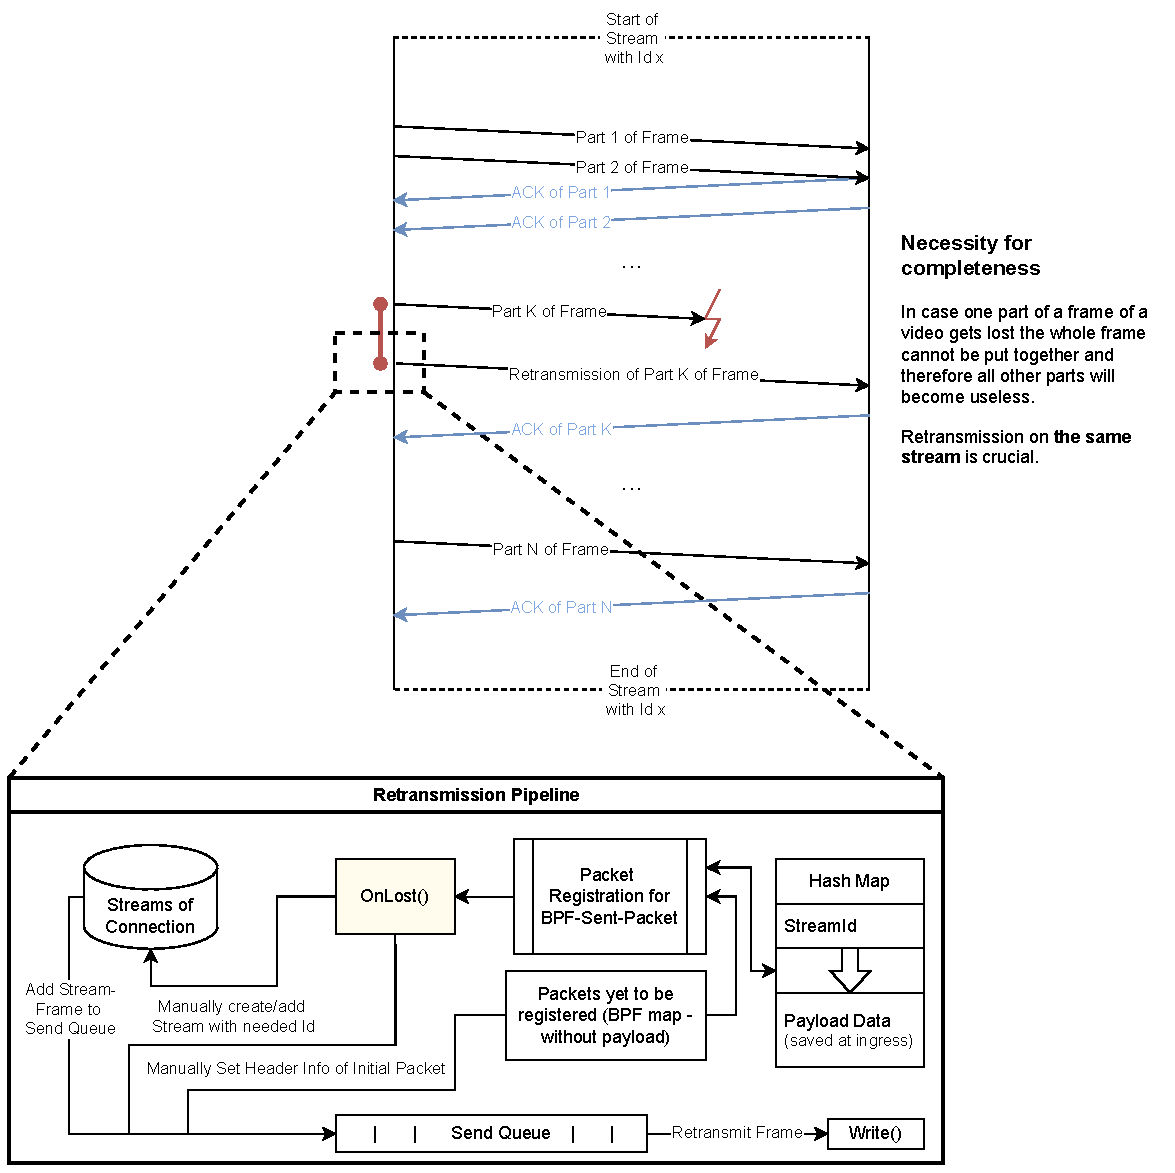
\includegraphics[width=\textwidth]{figures/03_fast_relays/retransmission.drawio.pdf}
    \caption[Packet retransmission schematic]{Internal setup for retransmitting packets forwarded from server connection.}\label{fig:packet-retransmission}
\end{figure}

It is not necessary to create the stream before that because our approach is only working with 
unidirectional streams so the relay does not get any data back from the client.
The only case where it matters that the relay state ``knows'' about the stream is when a packet
gets lost, and the \verb|OnLost| function of the QUIC library is called.
This is also the latest point in time when the relay can create the stream with the needed stream-id.
\autoref{fig:packet-retransmission} visualizes the setup for retransmitting a packet that 
got lost on its way to the client. 